\chapter{Análisis del sistema}
\label{ch:analisis}
En este capítulo se explica de qué es capaz el producto desarrollado. Comienza con una descripción del sistema de una manera detallada, a continuación se extraerán los requisitos de usuario y casos de uso, lo que nos permite hacernos una idea clara de lo que necesita el sistema y así poder conceptualizarlo en forma de requisitos de software. En último lugar, se establece la relación entre los requisitos de usuario y los de software en una matriz de trazabilidad, pudiendo así comprobar que todas las peticiones del usuario han sido tenidas en cuenta.

Además, este capítulo sirve como base para los siguientes, como son el de Diseño (\autoref{ch:diseno}) y el de Implementación (\autoref{ch:implementacion}), en los que basándose en los requisitos recogidos se empezara a dar forma al sistema.

\section{Definición del Sistema}\label{sec:definición-del-sistema}
El propósito de este proyecto es desarrollar un dispositivo que nos proporcione videovigilancia y medidas de diferentes factores ambientales, para garantizar la seguridad de un CPD. Las diferentes medidas que se tomen se almacenaran para poder ser consultadas junto con la imagen de videovigilancia a través de una plataforma web.
\begin{figure}[H]
	\ffigbox[\FBwidth]
	{\caption{Diagrama del sistema}
		\label{fig:diagrama_sistema}}
	{\tikzset{every picture/.style={line width=0.75pt}} %set default line width to 0.75pt        
	
	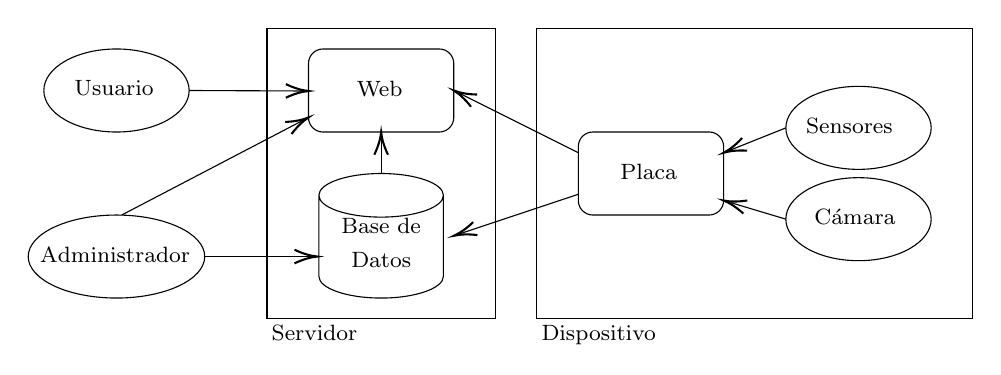
\begin{tikzpicture}[x=0.75pt,y=0.75pt,yscale=-1,xscale=1]
		
		\draw   (82.49,90) .. controls (82.49,78.95) and (98.16,70) .. (117.49,70) .. controls (136.82,70) and (152.49,78.95) .. (152.49,90) .. controls (152.49,101.05) and (136.82,110) .. (117.49,110) .. controls (98.16,110) and (82.49,101.05) .. (82.49,90) -- cycle ;
		
		\draw   (320,60) -- (530,60) -- (530,200) -- (320,200) -- cycle ;
		\draw   (440,108) .. controls (440,96.95) and (455.67,88) .. (475,88) .. controls (494.33,88) and (510,96.95) .. (510,108) .. controls (510,119.05) and (494.33,128) .. (475,128) .. controls (455.67,128) and (440,119.05) .. (440,108) -- cycle ;
		
		\draw   (275,140.5) -- (275,179.5) .. controls (275,185.3) and (261.57,190) .. (245,190) .. controls (228.43,190) and (215,185.3) .. (215,179.5) -- (215,140.5)(275,140.5) .. controls (275,146.3) and (261.57,151) .. (245,151) .. controls (228.43,151) and (215,146.3) .. (215,140.5) .. controls (215,134.7) and (228.43,130) .. (245,130) .. controls (261.57,130) and (275,134.7) .. (275,140.5) -- cycle ;
		
		\draw   (210,77) .. controls (210,73.13) and (213.13,70) .. (217,70) -- (273,70) .. controls (276.87,70) and (280,73.13) .. (280,77) -- (280,103) .. controls (280,106.87) and (276.87,110) .. (273,110) -- (217,110) .. controls (213.13,110) and (210,106.87) .. (210,103) -- cycle ;
		
		\draw   (340,117) .. controls (340,113.13) and (343.13,110) .. (347,110) -- (403,110) .. controls (406.87,110) and (410,113.13) .. (410,117) -- (410,143) .. controls (410,146.87) and (406.87,150) .. (403,150) -- (347,150) .. controls (343.13,150) and (340,146.87) .. (340,143) -- cycle ;
		
		\draw   (440,152) .. controls (440,140.95) and (455.67,132) .. (475,132) .. controls (494.33,132) and (510,140.95) .. (510,152) .. controls (510,163.05) and (494.33,172) .. (475,172) .. controls (455.67,172) and (440,163.05) .. (440,152) -- cycle ;
		
		\draw    (440,152) -- (411.92,143.57) ;
		\draw [shift={(410,143)}, rotate = 376.7] [color={rgb, 255:red, 0; green, 0; blue, 0 }  ][line width=0.75]    (10.93,-3.29) .. controls (6.95,-1.4) and (3.31,-0.3) .. (0,0) .. controls (3.31,0.3) and (6.95,1.4) .. (10.93,3.29)   ;
		\draw    (440,108) -- (411.86,119.26) ;
		\draw [shift={(410,120)}, rotate = 338.2] [color={rgb, 255:red, 0; green, 0; blue, 0 }  ][line width=0.75]    (10.93,-3.29) .. controls (6.95,-1.4) and (3.31,-0.3) .. (0,0) .. controls (3.31,0.3) and (6.95,1.4) .. (10.93,3.29)   ;
		\draw    (152.49,90) -- (208,90.24) ;
		\draw [shift={(210,90.25)}, rotate = 180.25] [color={rgb, 255:red, 0; green, 0; blue, 0 }  ][line width=0.75]    (10.93,-3.29) .. controls (6.95,-1.4) and (3.31,-0.3) .. (0,0) .. controls (3.31,0.3) and (6.95,1.4) .. (10.93,3.29)   ;
		\draw    (340,120) -- (281.79,90.89) ;
		\draw [shift={(280,90)}, rotate = 386.57] [color={rgb, 255:red, 0; green, 0; blue, 0 }  ][line width=0.75]    (10.93,-3.29) .. controls (6.95,-1.4) and (3.31,-0.3) .. (0,0) .. controls (3.31,0.3) and (6.95,1.4) .. (10.93,3.29)   ;
		\draw    (340,140) -- (281.9,159.37) ;
		\draw [shift={(280,160)}, rotate = 341.57] [color={rgb, 255:red, 0; green, 0; blue, 0 }  ][line width=0.75]    (10.93,-3.29) .. controls (6.95,-1.4) and (3.31,-0.3) .. (0,0) .. controls (3.31,0.3) and (6.95,1.4) .. (10.93,3.29)   ;
		\draw    (245,130) -- (245,112) ;
		\draw [shift={(245,110)}, rotate = 450] [color={rgb, 255:red, 0; green, 0; blue, 0 }  ][line width=0.75]    (10.93,-3.29) .. controls (6.95,-1.4) and (3.31,-0.3) .. (0,0) .. controls (3.31,0.3) and (6.95,1.4) .. (10.93,3.29)   ;
		\draw   (190,60) -- (300,60) -- (300,200) -- (190,200) -- cycle ;
		\draw   (74.97,170) .. controls (74.97,158.95) and (94.01,150) .. (117.49,150) .. controls (140.97,150) and (160,158.95) .. (160,170) .. controls (160,181.05) and (140.97,190) .. (117.49,190) .. controls (94.01,190) and (74.97,181.05) .. (74.97,170) -- cycle ;
		
		\draw    (160.2,170) -- (212.2,170) ;
		\draw [shift={(214.2,170)}, rotate = 180] [color={rgb, 255:red, 0; green, 0; blue, 0 }  ][line width=0.75]    (10.93,-3.29) .. controls (6.95,-1.4) and (3.31,-0.3) .. (0,0) .. controls (3.31,0.3) and (6.95,1.4) .. (10.93,3.29)   ;
		\draw    (120,150) -- (208.23,103.93) ;
		\draw [shift={(210,103)}, rotate = 512.4300000000001] [color={rgb, 255:red, 0; green, 0; blue, 0 }  ][line width=0.75]    (10.93,-3.29) .. controls (6.95,-1.4) and (3.31,-0.3) .. (0,0) .. controls (3.31,0.3) and (6.95,1.4) .. (10.93,3.29)   ;
		
		\draw (321,202) node [anchor=north west][inner sep=0.75pt]  [font=\footnotesize] [align=left] {Dispositivo};
		\draw (222,150.43) node [anchor=north west][inner sep=0.75pt]   [align=left] {\begin{minipage}[lt]{32.65pt}\setlength\topsep{0pt}
				\begin{center}
					{\footnotesize Base de}\\{\footnotesize Datos}
				\end{center}
				
			\end{minipage}};
		\draw (232,84) node [anchor=north west][inner sep=0.75pt]  [font=\footnotesize] [align=left] {Web};
		\draw (191,202) node [anchor=north west][inner sep=0.75pt]  [font=\footnotesize] [align=left] {Servidor};
		\draw (95.99,84) node [anchor=north west][inner sep=0.75pt]  [font=\footnotesize] [align=left] {Usuario};
		\draw (359,124) node [anchor=north west][inner sep=0.75pt]  [font=\footnotesize] [align=left] {Placa};
		\draw (448.5,102) node [anchor=north west][inner sep=0.75pt]  [font=\footnotesize] [align=left] {Sensores};
		\draw (452.5,146) node [anchor=north west][inner sep=0.75pt]  [font=\footnotesize] [align=left] {Cámara};
		\draw (79.49,164) node [anchor=north west][inner sep=0.75pt]  [font=\footnotesize] [align=left] {Administrador};
		
	\end{tikzpicture}}
\end{figure}

Como se puede ver en la \autoref{fig:diagrama_sistema} el sistema consistirá en:
\begin{itemize}
	\item \textbf{Usuario:} Será el personal autorizado encargado de controlar las imágenes que proporcione la cámara y revisar las mediciones que transmitan los sensores del dispositivo.
	\item \textbf{Administrador:} Persona encargada del mantenimiento de la Base de Datos y de la web, así como de la buena recepción de las mediciones y de las imágenes. Ante cualquier incidencia es el responsable de resolverla.
	\item \textbf{Web:} Página donde se puede acceder a los diferentes dispositivos, sus medidas e imagen de video.
	\item \textbf{Base de Datos:} Almacén de la información de los usuarios, la de los dispositivos y las mediciones que recogen.
	\item \textbf{Servidor:} Lugar accesible para el usuario donde se alojan la web y la base de datos.
	\item \textbf{Placa:} Dispositivo donde se implantan los distintos sensores y la cámara.
	\item \textbf{Sensores:} Dispositivos sensibles a los diferentes factores ambientales que se medirán en el CPD\@.
	\item \textbf{Cámara:} Dispositivo que captura la imagen que se utilizara para la videovigilancia.
	\item \textbf{Dispositivo:} Conjunto de la placa, los sensores y la cámara.
\end{itemize}

\section{Requisitos de usuario}\label{sec:requisitos-de-usuario}
En esta sección se recogen todas exigencias que el cliente nos solicita para este proyecto, en forma de requisitos de usuario, que serán mostrados según la \autoref{tab:plantilla_ru}.
\begin{table}[H]
	\centering
	\caption{Plantilla de los Requisitos de Usuario}
	\label{tab:plantilla_ru}
	\begin{tabular}{|l|p{.77\textwidth}|}
		\hline
		\multicolumn{2}{|c|}{\cellcolor[HTML]{BFBFBF}{\color[HTML]{000000} \textbf{RU-XX}}} \\ \hline
		\textbf{Nombre}      &   \\ \hline
		\textbf{Descripción} &   \\ \hline
		\textbf{Prioridad}   &   \\ \hline
		\textbf{Necesidad}   &   \\ \hline
		\textbf{Fuente}      &   \\ \hline
		\textbf{Versión}     &   \\ \hline
	\end{tabular}
\end{table}
\begin{itemize}
	\item \textbf{RU-XX:} Identificador del Requisito de Usuario, el XX tomará un valor en función de la posición.
	\item \textbf{Nombre:} Nombre representativo del asunto del requisito.
	\item \textbf{Descripción:} Exposición más detallada del requisito.
	\item \textbf{Prioridad:} Indica si debe ser considerado desde el principio o si, por el contrario, puede retrasarse. Puede ser: Alta, Mediana o Baja.
	\item \textbf{Necesidad:} Importancia del requisito sobre el sistema, pudiendo ser: Esencial, Deseable u Opcional.
	\item \textbf{Fuente:} Procedencia del requisito.
	\item \textbf{Versión:} Indica si ha sufrido variaciones a lo largo del tiempo.
\end{itemize}

Los requisitos de usuario son los siguientes:
\newcount\ru
\ru=1
\begin{table}[H]
	\caption{RU-0\number\ru}
	\begin{tabular}{|l|p{.77\textwidth}|}
		\hline
		\multicolumn{2}{|c|}{\cellcolor[HTML]{BFBFBF}{\color[HTML]{000000} \textbf{RU-0\number\ru}}} \\ \hline
		\textbf{Nombre}      & Medir la temperatura                                                                                          \\ \hline
		\textbf{Descripción} & El dispositivo debe contar con un sensor capaz medir la temperatura de la sala entre los valores establecidos \\ \hline
		\textbf{Prioridad}   & Alta                                                                                                          \\ \hline
		\textbf{Necesidad}   & Esencial                                                                                                      \\ \hline
		\textbf{Fuente}      & Cliente                                                                                                       \\ \hline
		\textbf{Versión}     & 1.0                                                                                                           \\ \hline
	\end{tabular}
\end{table}
\advance\ru by 1
\begin{table}[H]
	\caption{RU-0\number\ru}
	\begin{tabular}{|l|p{.77\textwidth}|}
		\hline
		\multicolumn{2}{|c|}{\cellcolor[HTML]{BFBFBF}{\color[HTML]{000000} \textbf{RU-0\number\ru}}} \\ \hline
		\textbf{Nombre}      & Medir la humedad                                                                                          \\ \hline
		\textbf{Descripción} & El dispositivo debe contar con un sensor capaz medir la humedad de la sala entre los valores establecidos \\ \hline
		\textbf{Prioridad}   & Alta                                                                                                      \\ \hline
		\textbf{Necesidad}   & Esencial                                                                                                  \\ \hline
		\textbf{Fuente}      & Cliente                                                                                                   \\ \hline
		\textbf{Versión}     & 1.0                                                                                                       \\ \hline
	\end{tabular}
\end{table}
\advance\ru by 1
\begin{table}[H]
	\caption{RU-0\number\ru}
	\begin{tabular}{|l|p{.77\textwidth}|}
		\hline
		\multicolumn{2}{|c|}{\cellcolor[HTML]{BFBFBF}{\color[HTML]{000000} \textbf{RU-0\number\ru}}} \\ \hline
		\textbf{Nombre}      & Medir el CO                                                                                                           \\ \hline
		\textbf{Descripción} & El dispositivo debe contar con un sensor capaz medir el monóxido de carbono de la sala entre los valores establecidos \\ \hline
		\textbf{Prioridad}   & Media                                                                                                                 \\ \hline
		\textbf{Necesidad}   & Deseable                                                                                                              \\ \hline
		\textbf{Fuente}      & Cliente                                                                                                               \\ \hline
		\textbf{Versión}     & 1.0                                                                                                                   \\ \hline
	\end{tabular}
\end{table}
\advance\ru by 1
\begin{table}[H]
	\caption{RU-0\number\ru}
	\begin{tabular}{|l|p{.77\textwidth}|}
		\hline
		\multicolumn{2}{|c|}{\cellcolor[HTML]{BFBFBF}{\color[HTML]{000000} \textbf{RU-0\number\ru}}} \\ \hline
		\textbf{Nombre}      & Medir el CO$_2$                                                                                                      \\ \hline
		\textbf{Descripción} & El dispositivo debe contar con un sensor capaz medir el dióxido de carbono de la sala entre los valores establecidos \\ \hline
		\textbf{Prioridad}   & Media                                                                                                                \\ \hline
		\textbf{Necesidad}   & Deseable                                                                                                             \\ \hline
		\textbf{Fuente}      & Cliente                                                                                                              \\ \hline
		\textbf{Versión}     & 1.0                                                                                                                  \\ \hline
	\end{tabular}
\end{table}
\advance\ru by 1
\begin{table}[H]
	\caption{RU-0\number\ru}
	\begin{tabular}{|l|p{.77\textwidth}|}
		\hline
		\multicolumn{2}{|c|}{\cellcolor[HTML]{BFBFBF}{\color[HTML]{000000} \textbf{RU-0\number\ru}}} \\ \hline
		\textbf{Nombre}      & Medir la calidad del aire                                                                                           \\ \hline
		\textbf{Descripción} & El dispositivo debe contar con un sensor capaz medir la calidad del aire de la sala para el correcto funcionamiento \\ \hline
		\textbf{Prioridad}   & Media                                                                                                               \\ \hline
		\textbf{Necesidad}   & Deseable                                                                                                            \\ \hline
		\textbf{Fuente}      & Cliente                                                                                                             \\ \hline
		\textbf{Versión}     & 1.0                                                                                                                 \\ \hline
	\end{tabular}
\end{table}
\advance\ru by 1
\begin{table}[H]
	\caption{RU-0\number\ru}
	\begin{tabular}{|l|p{.77\textwidth}|}
		\hline
		\multicolumn{2}{|c|}{\cellcolor[HTML]{BFBFBF}{\color[HTML]{000000} \textbf{RU-0\number\ru}}} \\ \hline
		\textbf{Nombre}      & Videovigilancia                                                              \\ \hline
		\textbf{Descripción} & El dispositivo debe captar la imagen del interior de la sala en todo momento \\ \hline
		\textbf{Prioridad}   & Alta                                                                         \\ \hline
		\textbf{Necesidad}   & Esencial                                                                     \\ \hline
		\textbf{Fuente}      & Cliente                                                                      \\ \hline
		\textbf{Versión}     & 1.0                                                                          \\ \hline
	\end{tabular}
\end{table}
\advance\ru by 1
\begin{table}[H]
	\caption{RU-0\number\ru}
	\begin{tabular}{|l|p{.77\textwidth}|}
		\hline
		\multicolumn{2}{|c|}{\cellcolor[HTML]{BFBFBF}{\color[HTML]{000000} \textbf{RU-0\number\ru}}} \\ \hline
		\textbf{Nombre}      & Conectividad                                            \\ \hline
		\textbf{Descripción} & El dispositivo debe tener conexión inalámbrica a la red \\ \hline
		\textbf{Prioridad}   & Alta                                                    \\ \hline
		\textbf{Necesidad}   & Esencial                                                \\ \hline
		\textbf{Fuente}      & Cliente                                                 \\ \hline
		\textbf{Versión}     & 1.0                                                     \\ \hline
	\end{tabular}
\end{table}
\advance\ru by 1
\begin{table}[H]
	\caption{RU-0\number\ru}
	\begin{tabular}{|l|p{.77\textwidth}|}
		\hline
		\multicolumn{2}{|c|}{\cellcolor[HTML]{BFBFBF}{\color[HTML]{000000} \textbf{RU-0\number\ru}}} \\ \hline
		\textbf{Nombre}      & Bajo consumo                                        \\ \hline
		\textbf{Descripción} & El dispositivo debe tener un bajo consumo eléctrico \\ \hline
		\textbf{Prioridad}   & Media                                               \\ \hline
		\textbf{Necesidad}   & Deseable                                            \\ \hline
		\textbf{Fuente}      & Cliente                                             \\ \hline
		\textbf{Versión}     & 1.0                                                 \\ \hline
	\end{tabular}
\end{table}
\advance\ru by 1
\begin{table}[H]
	\caption{RU-0\number\ru}
	\begin{tabular}{|l|p{.77\textwidth}|}
		\hline
		\multicolumn{2}{|c|}{\cellcolor[HTML]{BFBFBF}{\color[HTML]{000000} \textbf{RU-0\number\ru}}} \\ \hline
		\textbf{Nombre}      & Histórico de medidas                            \\ \hline
		\textbf{Descripción} & Se deben almacenar todas las medidas realizadas \\ \hline
		\textbf{Prioridad}   & Alta                                            \\ \hline
		\textbf{Necesidad}   & Esencial                                        \\ \hline
		\textbf{Fuente}      & Cliente                                         \\ \hline
		\textbf{Versión}     & 1.0                                             \\ \hline
	\end{tabular}
\end{table}
\advance\ru by 1
\begin{table}[H]
	\caption{RU-\number\ru}
	\begin{tabular}{|l|p{.77\textwidth}|}
		\hline
		\multicolumn{2}{|c|}{\cellcolor[HTML]{BFBFBF}{\color[HTML]{000000} \textbf{RU-\number\ru}}} \\ \hline
		\textbf{Nombre}      & Frecuencia de las medidas                                                \\ \hline
		\textbf{Descripción} & El dispositivo debe realizar las medidas con la mayor frecuencia posible \\ \hline
		\textbf{Prioridad}   & Media                                                                    \\ \hline
		\textbf{Necesidad}   & Deseable                                                                 \\ \hline
		\textbf{Fuente}      & Cliente                                                                  \\ \hline
		\textbf{Versión}     & 1.0                                                                      \\ \hline
	\end{tabular}
\end{table}
\advance\ru by 1
\begin{table}[H]
	\caption{RU-\number\ru}
	\begin{tabular}{|l|p{.77\textwidth}|}
		\hline
		\multicolumn{2}{|c|}{\cellcolor[HTML]{BFBFBF}{\color[HTML]{000000} \textbf{RU-\number\ru}}} \\ \hline
		\textbf{Nombre}      & Conexión con la web                                                                          \\ \hline
		\textbf{Descripción} & El dispositivo debe ser capaz de transmitir las medidas e imagen para que se vean  en la web \\ \hline
		\textbf{Prioridad}   & Media                                                                                        \\ \hline
		\textbf{Necesidad}   & Esencial                                                                                     \\ \hline
		\textbf{Fuente}      & Cliente                                                                                      \\ \hline
		\textbf{Versión}     & 1.0                                                                                          \\ \hline
	\end{tabular}
\end{table}
\advance\ru by 1
\begin{table}[H]
	\caption{RU-\number\ru}
	\begin{tabular}{|l|p{.77\textwidth}|}
		\hline
		\multicolumn{2}{|c|}{\cellcolor[HTML]{BFBFBF}{\color[HTML]{000000} \textbf{RU-\number\ru}}} \\ \hline
		\textbf{Nombre}      & Registro en la web                                                                                \\ \hline
		\textbf{Descripción} & El usuario debe solicitar al administrador del sistema que le conceda unas credenciales de acceso \\ \hline
		\textbf{Prioridad}   & Alta                                                                                              \\ \hline
		\textbf{Necesidad}   & Esencial                                                                                          \\ \hline
		\textbf{Fuente}      & Cliente                                                                                           \\ \hline
		\textbf{Versión}     & 1.0                                                                                               \\ \hline
	\end{tabular}
\end{table}
\advance\ru by 1
\begin{table}[H]
	\caption{RU-\number\ru}
	\begin{tabular}{|l|p{.77\textwidth}|}
		\hline
		\multicolumn{2}{|c|}{\cellcolor[HTML]{BFBFBF}{\color[HTML]{000000} \textbf{RU-\number\ru}}} \\ \hline
		\textbf{Nombre}      & Inicio de sesión                                                                                        \\ \hline
		\textbf{Descripción} & El usuario para acceder a la web debe aportar un usuario y contraseña que se le ha asignado previamente \\ \hline
		\textbf{Prioridad}   & Alta                                                                                                    \\ \hline
		\textbf{Necesidad}   & Esencial                                                                                                \\ \hline
		\textbf{Fuente}      & Cliente                                                                                                 \\ \hline
		\textbf{Versión}     & 1.0                                                                                                     \\ \hline
	\end{tabular}
\end{table}
\advance\ru by 1
\begin{table}[H]
	\caption{RU-\number\ru}
	\begin{tabular}{|l|p{.77\textwidth}|}
		\hline
		\multicolumn{2}{|c|}{\cellcolor[HTML]{BFBFBF}{\color[HTML]{000000} \textbf{RU-\number\ru}}} \\ \hline
		\textbf{Nombre}      & Seguridad de la contraseña                                                 \\ \hline
		\textbf{Descripción} & La contraseña se debe almacenar de manera segura ante posibles intrusiones \\ \hline
		\textbf{Prioridad}   & Media                                                                      \\ \hline
		\textbf{Necesidad}   & Deseable                                                                   \\ \hline
		\textbf{Fuente}      & Cliente                                                                    \\ \hline
		\textbf{Versión}     & 1.0                                                                        \\ \hline
	\end{tabular}
\end{table}
\advance\ru by 1
\begin{table}[H]
	\caption{RU-\number\ru}
	\begin{tabular}{|l|p{.77\textwidth}|}
		\hline
		\multicolumn{2}{|c|}{\cellcolor[HTML]{BFBFBF}{\color[HTML]{000000} \textbf{RU-\number\ru}}} \\ \hline
		\textbf{Nombre}      & Lista de dispositivos                                                                                   \\ \hline
		\textbf{Descripción} & Cuando el usuario este dentro de su cuenta podrá ver los diferentes dispositivos a los que tiene acceso \\ \hline
		\textbf{Prioridad}   & Baja                                                                                                    \\ \hline
		\textbf{Necesidad}   & Opcional                                                                                                \\ \hline
		\textbf{Fuente}      & Cliente                                                                                                 \\ \hline
		\textbf{Versión}     & 1.0                                                                                                     \\ \hline
	\end{tabular}
\end{table}
\advance\ru by 1
\begin{table}[H]
	\caption{RU-\number\ru}
	\begin{tabular}{|l|p{.77\textwidth}|}
		\hline
		\multicolumn{2}{|c|}{\cellcolor[HTML]{BFBFBF}{\color[HTML]{000000} \textbf{RU-\number\ru}}} \\ \hline
		\textbf{Nombre}      & Cerrar sesión                        \\ \hline
		\textbf{Descripción} & El usuario podrá salir de su cuenta. \\ \hline
		\textbf{Prioridad}   & Alta                                 \\ \hline
		\textbf{Necesidad}   & Esencial                             \\ \hline
		\textbf{Fuente}      & Cliente                              \\ \hline
		\textbf{Versión}     & 1.0                                  \\ \hline
	\end{tabular}
\end{table}
\advance\ru by 1
\begin{table}[H]
	\caption{RU-\number\ru}
	\begin{tabular}{|l|p{.77\textwidth}|}
		\hline
		\multicolumn{2}{|c|}{\cellcolor[HTML]{BFBFBF}{\color[HTML]{000000} \textbf{RU-\number\ru}}} \\ \hline
		\textbf{Nombre}      & Verificar nombre de usuario                                                          \\ \hline
		\textbf{Descripción} & Al acceder el usuario podrá ver su nombre de usuario para comprobar que es su cuenta \\ \hline
		\textbf{Prioridad}   & Baja                                                                                 \\ \hline
		\textbf{Necesidad}   & Opcional                                                                             \\ \hline
		\textbf{Fuente}      & Cliente                                                                              \\ \hline
		\textbf{Versión}     & 1.0                                                                                  \\ \hline
	\end{tabular}
\end{table}
\advance\ru by 1
\begin{table}[H]
	\caption{RU-\number\ru}
	\begin{tabular}{|l|p{.77\textwidth}|}
		\hline
		\multicolumn{2}{|c|}{\cellcolor[HTML]{BFBFBF}{\color[HTML]{000000} \textbf{RU-\number\ru}}} \\ \hline
		\textbf{Nombre}      & Colores de la web                                                                                   \\ \hline
		\textbf{Descripción} & La web debe estar diseñada en colores no estridentes para que se puedan ver bien en cualquier lugar \\ \hline
		\textbf{Prioridad}   & Alta                                                                                                \\ \hline
		\textbf{Necesidad}   & Deseable                                                                                            \\ \hline
		\textbf{Fuente}      & Cliente                                                                                             \\ \hline
		\textbf{Versión}     & 1.0                                                                                                 \\ \hline
	\end{tabular}
\end{table}
\advance\ru by 1
\begin{table}[H]
	\caption{RU-\number\ru}
	\begin{tabular}{|l|p{.77\textwidth}|}
		\hline
		\multicolumn{2}{|c|}{\cellcolor[HTML]{BFBFBF}{\color[HTML]{000000} \textbf{RU-\number\ru}}} \\ \hline
		\textbf{Nombre}      & Acceso a la web                                                                   \\ \hline
		\textbf{Descripción} & La web debe poder ser accesible desde cualquier dispositivo con acceso a internet \\ \hline
		\textbf{Prioridad}   & Alta                                                                              \\ \hline
		\textbf{Necesidad}   & Esencial                                                                          \\ \hline
		\textbf{Fuente}      & Cliente                                                                           \\ \hline
		\textbf{Versión}     & 1.0                                                                               \\ \hline
	\end{tabular}
\end{table}
\advance\ru by 1
\begin{table}[H]
	\caption{RU-\number\ru}
	\begin{tabular}{|l|p{.77\textwidth}|}
		\hline
		\multicolumn{2}{|c|}{\cellcolor[HTML]{BFBFBF}{\color[HTML]{000000} \textbf{RU-\number\ru}}} \\ \hline
		\textbf{Nombre}      & Página de dispositivo                                                     \\ \hline
		\textbf{Descripción} & Cuando se accede a un dispositivo se mostrará la imagen y medidas tomadas \\ \hline
		\textbf{Prioridad}   & Alta                                                                      \\ \hline
		\textbf{Necesidad}   & Esencial                                                                  \\ \hline
		\textbf{Fuente}      & Cliente                                                                   \\ \hline
		\textbf{Versión}     & 1.0                                                                       \\ \hline
	\end{tabular}
\end{table}
\advance\ru by 1
\begin{table}[H]
	\caption{RU-\number\ru}
	\begin{tabular}{|l|p{.77\textwidth}|}
		\hline
		\multicolumn{2}{|c|}{\cellcolor[HTML]{BFBFBF}{\color[HTML]{000000} \textbf{RU-\number\ru}}} \\ \hline
		\textbf{Nombre}      & Imagen de la cámara                                                                            \\ \hline
		\textbf{Descripción} & La imagen de la cámara debe ser tomada en todo momento, mientras el dispositivo esté conectado \\ \hline
		\textbf{Prioridad}   & Alta                                                                                           \\ \hline
		\textbf{Necesidad}   & Esencial                                                                                       \\ \hline
		\textbf{Fuente}      & Cliente                                                                                        \\ \hline
		\textbf{Versión}     & 1.0                                                                                            \\ \hline
	\end{tabular}
\end{table}
\advance\ru by 1
\begin{table}[H]
	\caption{RU-\number\ru}
	\begin{tabular}{|l|p{.77\textwidth}|}
		\hline
		\multicolumn{2}{|c|}{\cellcolor[HTML]{BFBFBF}{\color[HTML]{000000} \textbf{RU-\number\ru}}} \\ \hline
		\textbf{Nombre}      & Navegar entre las medidas                                                                                                   \\ \hline
		\textbf{Descripción} & Cuando se está en una página de dispositivo, el usuario, debe poder moverse con facilidad entre todos los datos registrados \\ \hline
		\textbf{Prioridad}   & Media                                                                                                                       \\ \hline
		\textbf{Necesidad}   & Deseable                                                                                                                    \\ \hline
		\textbf{Fuente}      & Cliente                                                                                                                     \\ \hline
		\textbf{Versión}     & 1.0                                                                                                                         \\ \hline
	\end{tabular}
\end{table}
\advance\ru by 1
\begin{table}[H]
	\caption{RU-\number\ru}
	\begin{tabular}{|l|p{.77\textwidth}|}
		\hline
		\multicolumn{2}{|c|}{\cellcolor[HTML]{BFBFBF}{\color[HTML]{000000} \textbf{RU-\number\ru}}} \\ \hline
		\textbf{Nombre}      & Medidas tomadas                                                                                      \\ \hline
		\textbf{Descripción} & Los datos que tome el dispositivo deben mostrarse en varios formatos para facilitar su entendimiento \\ \hline
		\textbf{Prioridad}   & Baja                                                                                                 \\ \hline
		\textbf{Necesidad}   & Deseable                                                                                             \\ \hline
		\textbf{Fuente}      & Cliente                                                                                              \\ \hline
		\textbf{Versión}     & 1.0                                                                                                  \\ \hline
	\end{tabular}
\end{table}
\advance\ru by 1
\pagebreak

\section{Casos de uso}\label{sec:casos-de-uso}
En la \autoref{fig:diagrama_casos_uso} que se muestra a continuación se resumen todos los casos de uso del sistema.

\begin{figure}[H]
	\ffigbox[\textwidth]
	{\caption{Diagrama de Casos de Uso}
		\label{fig:diagrama_casos_uso}}
	{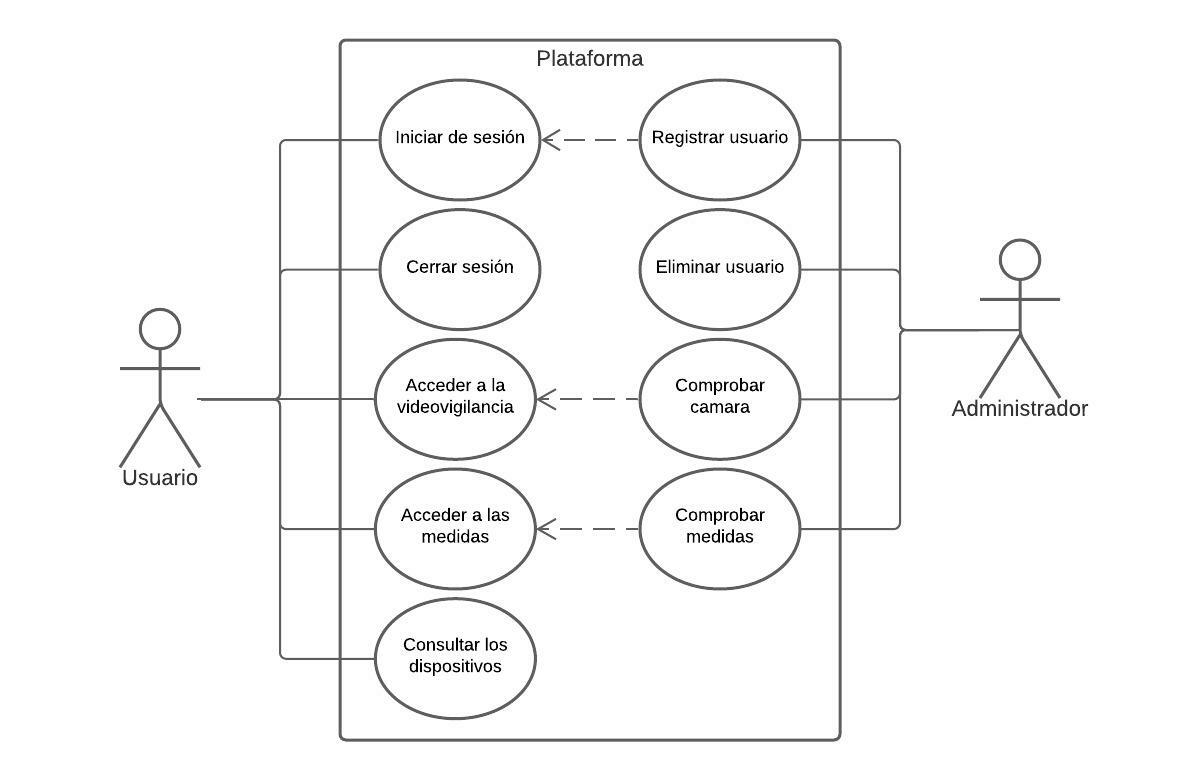
\includegraphics[width=\textwidth]{casos-de-uso.jpeg}}
\end{figure}

Para realizar una descripción más detallada de los casos de uso, empleamos la representación tabular que se muestra en la \autoref{tab:plantilla_cu}.
\begin{table}[H]
	\centering
	\caption{Plantilla de los Casos de Uso}
	\label{tab:plantilla_cu}
	\begin{tabular}{|l|p{.75\textwidth}|}
		\hline
		\multicolumn{2}{|c|}{\cellcolor[HTML]{BFBFBF}{\color[HTML]{000000} \textbf{CU-XX}}} \\ \hline
		\textbf{Caso de uso}     &   \\ \hline
		\textbf{Actores}         &   \\ \hline
		\textbf{Descripción}     &   \\ \hline
		\textbf{Precondiciones}  &   \\ \hline
		\textbf{Postcondiciones} &   \\ \hline
	\end{tabular}
\end{table}

\begin{itemize}
	\item \textbf{CU-XX:} Identificador del caso de uso, el XX tomará un valor en función del orden de este.
	\item \textbf{Caso de uso:} Nombre que identifica el caso de uso.
	\item \textbf{Actores:} Partes implicadas en el caso de uso.
	\item \textbf{Descripción:} Breve exposición de la situación.
	\item \textbf{Precondiciones:} Condiciones que se deben cumplir para que tenga lugar el caso de uso.
	\item \textbf{Postcondiciones:} Que ocurre si se cumple el caso de uso.
\end{itemize}

Ahora que entendemos el significado de cada una de las casillas se procede a detallar los casos de uso.
\newcount\cu
\cu=1
\begin{table}[H]
	\centering
	\caption{CU-0\number\cu}
	\begin{tabular}{|l|p{.75\textwidth}|}
		\hline
		\multicolumn{2}{|c|}{\cellcolor[HTML]{BFBFBF}{\color[HTML]{000000} \textbf{CU-0\number\cu}}} \\ \hline
		\textbf{Caso de uso}     & Registrar usuario                                          \\ \hline
		\textbf{Actores}         & Administrador                                              \\ \hline
		\textbf{Descripción}     & Crear un usuario y contraseña para acceder a la plataforma \\ \hline
		\textbf{Precondiciones}  & Acceder a la página de administración de la BBDD           \\ \hline
		\textbf{Postcondiciones} & Generación de usuario y contraseña de acceso               \\ \hline
	\end{tabular}
\end{table}
\advance\cu by 1
\begin{table}[H]
	\centering
	\caption{CU-0\number\cu}
	\begin{tabular}{|l|p{.75\textwidth}|}
		\hline
		\multicolumn{2}{|c|}{\cellcolor[HTML]{BFBFBF}{\color[HTML]{000000} \textbf{CU-0\number\cu}}} \\ \hline
		\textbf{Caso de uso}     & Eliminar usuario                                 \\ \hline
		\textbf{Actores}         & Administrador                                    \\ \hline
		\textbf{Descripción}     & Revocar el acceso a la plataforma                \\ \hline
		\textbf{Precondiciones}  & Acceder a la página de administración de la BBDD \\ \hline
		\textbf{Postcondiciones} & Registro de la tabla ‘user’ eliminado            \\ \hline
	\end{tabular}
\end{table}
\advance\cu by 1
\begin{table}[H]
	\centering
	\caption{CU-0\number\cu}
	\begin{tabular}{|l|p{.75\textwidth}|}
		\hline
		\multicolumn{2}{|c|}{\cellcolor[HTML]{BFBFBF}{\color[HTML]{000000} \textbf{CU-0\number\cu}}} \\ \hline
		\textbf{Caso de uso}     & Comprobar medidas                                                                         \\ \hline
		\textbf{Actores}         & Administrador                                                                             \\ \hline
		\textbf{Descripción}     & Consultar las medidas, ver que los valores sean razonables y que se reciben continuamente \\ \hline
		\textbf{Precondiciones}  & Poseer usuario y clave de acceso de la BBDD                                               \\ \hline
		\textbf{Postcondiciones} & El administrador ha verificado que funciona correctamente                                 \\ \hline
	\end{tabular}
\end{table}
\advance\cu by 1
\begin{table}[H]
	\centering
	\caption{CU-0\number\cu}
	\begin{tabular}{|l|p{.75\textwidth}|}
		\hline
		\multicolumn{2}{|c|}{\cellcolor[HTML]{BFBFBF}{\color[HTML]{000000} \textbf{CU-0\number\cu}}} \\ \hline
		\textbf{Caso de uso}     & Comprobar cámara                                          \\ \hline
		\textbf{Actores}         & Administrador                                             \\ \hline
		\textbf{Descripción}     & Comprobar que la imagen de la cámara se ve y se actualiza \\ \hline
		\textbf{Precondiciones}  & Poseer usuario y clave de acceso a la web                 \\ \hline
		\textbf{Postcondiciones} & El administrador ha verificado que funciona correctamente \\ \hline
	\end{tabular}
\end{table}
\advance\cu by 1
\begin{table}[H]
	\centering
	\caption{CU-0\number\cu}
	\begin{tabular}{|l|p{.75\textwidth}|}
		\hline
		\multicolumn{2}{|c|}{\cellcolor[HTML]{BFBFBF}{\color[HTML]{000000} \textbf{CU-0\number\cu}}} \\ \hline
		\textbf{Caso de uso}     & Iniciar sesión                          \\ \hline
		\textbf{Actores}         & Usuario                                 \\ \hline
		\textbf{Descripción}     & Acceder a la aplicación                 \\ \hline
		\textbf{Precondiciones}  & El usuario y contraseña está registrado \\ \hline
		\textbf{Postcondiciones} & El usuario accede a la plataforma       \\ \hline
	\end{tabular}
\end{table}
\advance\cu by 1
\begin{table}[H]
	\centering
	\caption{CU-0\number\cu}
	\begin{tabular}{|l|p{.75\textwidth}|}
		\hline
		\multicolumn{2}{|c|}{\cellcolor[HTML]{BFBFBF}{\color[HTML]{000000} \textbf{CU-0\number\cu}}} \\ \hline
		\textbf{Caso de uso}     & Cerrar sesión                                                   \\ \hline
		\textbf{Actores}         & Usuario                                                         \\ \hline
		\textbf{Descripción}     & El usuario termina de consultar las medidas y sale de su cuenta \\ \hline
		\textbf{Precondiciones}  & El usuario ha iniciado sesión                                   \\ \hline
		\textbf{Postcondiciones} & El usuario vuelve a la pantalla de inicio de sesión             \\ \hline
	\end{tabular}
\end{table}
\advance\cu by 1
\begin{table}[H]
	\centering
	\caption{CU-0\number\cu}
	\begin{tabular}{|l|p{.75\textwidth}|}
		\hline
		\multicolumn{2}{|c|}{\cellcolor[HTML]{BFBFBF}{\color[HTML]{000000} \textbf{CU-0\number\cu}}} \\ \hline
		\textbf{Caso de uso}     & Consultar los dispositivos                                \\ \hline
		\textbf{Actores}         & Usuario                                                   \\ \hline
		\textbf{Descripción}     & Visualizar los diferentes dispositivos conectados         \\ \hline
		\textbf{Precondiciones}  & El usuario ha iniciado sesión                             \\ \hline
		\textbf{Postcondiciones} & El usuario visualiza los dispositivos, su estado y nombre \\ \hline
	\end{tabular}
\end{table}
\advance\cu by 1
\begin{table}[H]
	\centering
	\caption{CU-0\number\cu}
	\begin{tabular}{|l|p{.75\textwidth}|}
		\hline
		\multicolumn{2}{|c|}{\cellcolor[HTML]{BFBFBF}{\color[HTML]{000000} \textbf{CU-0\number\cu}}} \\ \hline
		\textbf{Caso de uso}     & Acceder a las medidas                                                                             \\ \hline
		\textbf{Actores}         & Usuario                                                                                           \\ \hline
		\textbf{Descripción}     & Consultar las diferentes medidas tomadas por el dispositivo                                       \\ \hline
		\textbf{Precondiciones}  & El usuario ha iniciado sesión y selecciona un dispositivo                                         \\ \hline
		\textbf{Postcondiciones} & El usuario accede a una página con las gráficas de las medidas y la tabla de histórico de medidas \\ \hline
	\end{tabular}
\end{table}
\advance\cu by 1
\begin{table}[H]
	\centering
	\caption{CU-0\number\cu}
	\begin{tabular}{|l|p{.75\textwidth}|}
		\hline
		\multicolumn{2}{|c|}{\cellcolor[HTML]{BFBFBF}{\color[HTML]{000000} \textbf{CU-0\number\cu}}} \\ \hline
		\textbf{Caso de uso}     & Acceder a la videovigilancia                                            \\ \hline
		\textbf{Actores}         & Usuario                                                                 \\ \hline
		\textbf{Descripción}     & Consultar la imagen de la cámara                                        \\ \hline
		\textbf{Precondiciones}  & El usuario ha iniciado sesión y selecciona un dispositivo               \\ \hline
		\textbf{Postcondiciones} & El usuario accede a una página con la imagen de la cámara a tiempo real \\ \hline
	\end{tabular}
\end{table}

\section{Requisitos de software}\label{sec:requisitos-de-software}
Los requisitos de software descritos en esta sección se basan en los requisitos de usuario proporcionados por el cliente y los casos de uso asociados al sistema. La plantilla que se sigue es la definida por la \autoref{tab:plantilla_rf_rn}.
\begin{table}[H]
	\caption{Plantilla de los Requisitos Funcionales y No funcionales}
	\label{tab:plantilla_rf_rn}
	\begin{tabular}{|l|p{.77\textwidth}|}
		\hline
		\multicolumn{2}{|c|}{\cellcolor[HTML]{BFBFBF}{\color[HTML]{000000} \textbf{ID-XX}}} \\ \hline
		\textbf{Nombre}      &   \\ \hline
		\textbf{Descripción} &   \\ \hline
		\textbf{Prioridad}   &   \\ \hline
		\textbf{Necesidad}   &   \\ \hline
		\textbf{Fuente}      &   \\ \hline
		\textbf{Versión}     &   \\ \hline
	\end{tabular}
\end{table}
\begin{itemize}
	\item \textbf{ID-XX:} Identifica los requisitos mediante la siguiente codificación: ID será RF si es un requisito funcional o RN si es un requisito no funcional y XX tomará un valor en función de la posición.
	\item \textbf{Nombre:} Nombre representativo del asunto del requisito.
	\item \textbf{Descripción:} Exposición más detallada del requisito.
	\item \textbf{Prioridad:} Indica si debe ser considerado desde el principio o si, por el contrario, puede retrasarse. Puede ser: Alta, Mediana o Baja.
	\item \textbf{Necesidad:} Importancia del requisito sobre el sistema, pudiendo ser: Esencial, Deseable u Opcional.
	\item \textbf{Fuente:} Procedencia del requisito.
	\item \textbf{Versión:} Indica si ha sufrido variaciones a lo largo del tiempo.
\end{itemize}

Tras esta explicación de la plantilla en las siguientes subsecciones se presentan los requisitos funcionales y no funcionales.
\subsection{Requisitos Funcionales}\label{subsec:requisitos-funcionales}
\newcount\rf
\rf=1
\begin{table}[H]
	\caption{RF-0\number\rf}
	\begin{tabular}{|l|p{.77\textwidth}|}
		\hline
		\multicolumn{2}{|c|}{\cellcolor[HTML]{BFBFBF}{\color[HTML]{000000} \textbf{RF-0\number\rf}}} \\ \hline
		\textbf{Nombre}      & Almacenamiento de medidas                                             \\ \hline
		\textbf{Descripción} & Todas las medidas tomadas por el dispositivo deben quedar registradas \\ \hline
		\textbf{Prioridad}   & Alta                                                                  \\ \hline
		\textbf{Necesidad}   & Esencial                                                              \\ \hline
		\textbf{Fuente}      & Cliente                                                               \\ \hline
		\textbf{Versión}     & 1.0                                                                   \\ \hline
	\end{tabular}
\end{table}
\advance\rf by 1
\begin{table}[H]
	\caption{RF-0\number\rf}
	\begin{tabular}{|l|p{.77\textwidth}|}
		\hline
		\multicolumn{2}{|c|}{\cellcolor[HTML]{BFBFBF}{\color[HTML]{000000} \textbf{RF-0\number\rf}}} \\ \hline
		\textbf{Nombre}      & Medidas dispositivo-web                                                    \\ \hline
		\textbf{Descripción} & Las medidas tomadas deben ser transmitidas para ser visualizadas en la web \\ \hline
		\textbf{Prioridad}   & Alta                                                                       \\ \hline
		\textbf{Necesidad}   & Esencial                                                                   \\ \hline
		\textbf{Fuente}      & Cliente                                                                    \\ \hline
		\textbf{Versión}     & 1.0                                                                        \\ \hline
	\end{tabular}
\end{table}
\advance\rf by 1
\begin{table}[H]
	\caption{RF-0\number\rf}
	\begin{tabular}{|l|p{.77\textwidth}|}
		\hline
		\multicolumn{2}{|c|}{\cellcolor[HTML]{BFBFBF}{\color[HTML]{000000} \textbf{RF-0\number\rf}}} \\ \hline
		\textbf{Nombre}      & Imagen cámara-web                                                            \\ \hline
		\textbf{Descripción} & Las imágenes de la cámara del dispositivo deben poder ser vista desde la web \\ \hline
		\textbf{Prioridad}   & Alta                                                                         \\ \hline
		\textbf{Necesidad}   & Esencial                                                                     \\ \hline
		\textbf{Fuente}      & Cliente                                                                      \\ \hline
		\textbf{Versión}     & 1.0                                                                          \\ \hline
	\end{tabular}
\end{table}
\advance\rf by 1
\begin{table}[H]
	\caption{RF-0\number\rf}
	\begin{tabular}{|l|p{.77\textwidth}|}
		\hline
		\multicolumn{2}{|c|}{\cellcolor[HTML]{BFBFBF}{\color[HTML]{000000} \textbf{RF-0\number\rf}}} \\ \hline
		\textbf{Nombre}      & Registro                                                                           \\ \hline
		\textbf{Descripción} & Los usuarios para acceder al sistema deben solicitar credenciales al administrador \\ \hline
		\textbf{Prioridad}   & Alta                                                                               \\ \hline
		\textbf{Necesidad}   & Esencial                                                                           \\ \hline
		\textbf{Fuente}      & Cliente                                                                            \\ \hline
		\textbf{Versión}     & 1.0                                                                                \\ \hline
	\end{tabular}
\end{table}
\advance\rf by 1
\begin{table}[H]
	\caption{RF-0\number\rf}
	\begin{tabular}{|l|p{.77\textwidth}|}
		\hline
		\multicolumn{2}{|c|}{\cellcolor[HTML]{BFBFBF}{\color[HTML]{000000} \textbf{RF-0\number\rf}}} \\ \hline
		\textbf{Nombre}      & Inicio de sesión                                                                                                       \\ \hline
		\textbf{Descripción} & Si el usuario está registrado, se podrá identificar mediante su nombre de usuario y contraseña para acceder al sistema \\ \hline
		\textbf{Prioridad}   & Alta                                                                                                                   \\ \hline
		\textbf{Necesidad}   & Esencial                                                                                                               \\ \hline
		\textbf{Fuente}      & Cliente                                                                                                                \\ \hline
		\textbf{Versión}     & 1.0                                                                                                                    \\ \hline
	\end{tabular}
\end{table}
\advance\rf by 1
\begin{table}[H]
	\caption{RF-0\number\rf}
	\begin{tabular}{|l|p{.77\textwidth}|}
		\hline
		\multicolumn{2}{|c|}{\cellcolor[HTML]{BFBFBF}{\color[HTML]{000000} \textbf{RF-0\number\rf}}} \\ \hline
		\textbf{Nombre}      & Lista de dispositivos                                                                                                                   \\ \hline
		\textbf{Descripción} & Al acceder el usuario podrá ver un listado de dispositivo con su nombre, estado, último cambio de estado y un botón para acceder a este \\ \hline
		\textbf{Prioridad}   & Alta                                                                                                                                    \\ \hline
		\textbf{Necesidad}   & Esencial                                                                                                                                \\ \hline
		\textbf{Fuente}      & Cliente                                                                                                                                 \\ \hline
		\textbf{Versión}     & 1.0                                                                                                                                     \\ \hline
	\end{tabular}
\end{table}
\advance\rf by 1
\begin{table}[H]
	\caption{RF-0\number\rf}
	\begin{tabular}{|l|p{.77\textwidth}|}
		\hline
		\multicolumn{2}{|c|}{\cellcolor[HTML]{BFBFBF}{\color[HTML]{000000} \textbf{RF-0\number\rf}}} \\ \hline
		\textbf{Nombre}      & Botón cerrar sesión                                                                                                                                                \\ \hline
		\textbf{Descripción} & En la parte inferior de todas las páginas aparecerá el botón ‘Cerrar sesión’ que devolverá al usuario a la página de inicio de sesión, habiendo olvidado su sesión \\ \hline
		\textbf{Prioridad}   & Alta                                                                                                                                                               \\ \hline
		\textbf{Necesidad}   & Esencial                                                                                                                                                           \\ \hline
		\textbf{Fuente}      & Analista                                                                                                                                                           \\ \hline
		\textbf{Versión}     & 1.0                                                                                                                                                                \\ \hline
	\end{tabular}
\end{table}
\advance\rf by 1
\begin{table}[H]
	\caption{RF-0\number\rf}
	\begin{tabular}{|l|p{.77\textwidth}|}
		\hline
		\multicolumn{2}{|c|}{\cellcolor[HTML]{BFBFBF}{\color[HTML]{000000} \textbf{RF-0\number\rf}}} \\ \hline
		\textbf{Nombre}      & Bienvenida a la web                                                                                   \\ \hline
		\textbf{Descripción} & Al acceder a la web el usuario podrá ver su nombre para comprobar que ha iniciado con éxito la sesión \\ \hline
		\textbf{Prioridad}   & Baja                                                                                                  \\ \hline
		\textbf{Necesidad}   & Opcional                                                                                              \\ \hline
		\textbf{Fuente}      & Cliente                                                                                               \\ \hline
		\textbf{Versión}     & 1.0                                                                                                   \\ \hline
	\end{tabular}
\end{table}
\advance\rf by 1
\begin{table}[H]
	\caption{RF-0\number\rf}
	\begin{tabular}{|l|p{.77\textwidth}|}
		\hline
		\multicolumn{2}{|c|}{\cellcolor[HTML]{BFBFBF}{\color[HTML]{000000} \textbf{RF-0\number\rf}}} \\ \hline
		\textbf{Nombre}      & Acceso a la web                                                               \\ \hline
		\textbf{Descripción} & Con el correspondiente enlace se debe poder acceder a la web dentro de la red \\ \hline
		\textbf{Prioridad}   & Alta                                                                          \\ \hline
		\textbf{Necesidad}   & Esencial                                                                      \\ \hline
		\textbf{Fuente}      & Cliente                                                                       \\ \hline
		\textbf{Versión}     & 1.0                                                                           \\ \hline
	\end{tabular}
\end{table}
\advance\rf by 1
\begin{table}[H]
	\caption{RF-\number\rf}
	\begin{tabular}{|l|p{.77\textwidth}|}
		\hline
		\multicolumn{2}{|c|}{\cellcolor[HTML]{BFBFBF}{\color[HTML]{000000} \textbf{RF-\number\rf}}} \\ \hline
		\textbf{Nombre}      & Página de dispositivo                                                                                                                         \\ \hline
		\textbf{Descripción} & Una vez el usuario ha elegido un dispositivo de la lista de dispositivos, se le llevará a su página donde estarán las medidas e imagen tomada \\ \hline
		\textbf{Prioridad}   & Alta                                                                                                                                          \\ \hline
		\textbf{Necesidad}   & Esencial                                                                                                                                      \\ \hline
		\textbf{Fuente}      & Cliente                                                                                                                                       \\ \hline
		\textbf{Versión}     & 1.0                                                                                                                                           \\ \hline
	\end{tabular}
\end{table}
\advance\rf by 1
\begin{table}[H]
	\caption{RF-\number\rf}
	\begin{tabular}{|l|p{.77\textwidth}|}
		\hline
		\multicolumn{2}{|c|}{\cellcolor[HTML]{BFBFBF}{\color[HTML]{000000} \textbf{RF-\number\rf}}} \\ \hline
		\textbf{Nombre}      & Botón volver                                                                                                                                                     \\ \hline
		\textbf{Descripción} & Cuando se está en una página de dispositivo debe poderse volver a la lista de dispositivos mediante un botón ‘Volver’ que se distribuyen a lo largo de la página \\ \hline
		\textbf{Prioridad}   & Media                                                                                                                                                            \\ \hline
		\textbf{Necesidad}   & Deseable                                                                                                                                                         \\ \hline
		\textbf{Fuente}      & Analista                                                                                                                                                         \\ \hline
		\textbf{Versión}     & 1.0                                                                                                                                                              \\ \hline
	\end{tabular}
\end{table}
\advance\rf by 1
\begin{table}[H]
	\caption{RF-\number\rf}
	\begin{tabular}{|l|p{.77\textwidth}|}
		\hline
		\multicolumn{2}{|c|}{\cellcolor[HTML]{BFBFBF}{\color[HTML]{000000} \textbf{RF-\number\rf}}} \\ \hline
		\textbf{Nombre}      & Medidas tomadas en tabla                                                                                                          \\ \hline
		\textbf{Descripción} & Los datos que tome el dispositivo deben mostrarse en forma tabular con los datos concretos para las medidas a lo largo del tiempo \\ \hline
		\textbf{Prioridad}   & Alta                                                                                                                              \\ \hline
		\textbf{Necesidad}   & Esencial                                                                                                                          \\ \hline
		\textbf{Fuente}      & Analista                                                                                                                          \\ \hline
		\textbf{Versión}     & 1.0                                                                                                                               \\ \hline
	\end{tabular}
\end{table}
\advance\rf by 1
\begin{table}[H]
	\caption{RF-\number\rf}
	\begin{tabular}{|l|p{.77\textwidth}|}
		\hline
		\multicolumn{2}{|c|}{\cellcolor[HTML]{BFBFBF}{\color[HTML]{000000} \textbf{RF-\number\rf}}} \\ \hline
		\textbf{Nombre}      & Gráfica de las medidas tomadas                                                                       \\ \hline
		\textbf{Descripción} & Los datos que tome el dispositivo se mostraran de manera gráfica para ver la progresión en el tiempo \\ \hline
		\textbf{Prioridad}   & Baja                                                                                                 \\ \hline
		\textbf{Necesidad}   & Deseable                                                                                             \\ \hline
		\textbf{Fuente}      & Analista                                                                                             \\ \hline
		\textbf{Versión}     & 1.0                                                                                                  \\ \hline
	\end{tabular}
\end{table}

\subsection{Requisitos No Funcionales}\label{subsec:requisitos-no-funcionales}
\newcount\rn
\rn=1
\begin{table}[H]
	\caption{RN-0\number\rn}
	\begin{tabular}{|l|p{.77\textwidth}|}
		\hline
		\multicolumn{2}{|c|}{\cellcolor[HTML]{BFBFBF}{\color[HTML]{000000} \textbf{RN-0\number\rn}}} \\ \hline
		\textbf{Nombre}      & Sensor de temperatura                                                                            \\ \hline
		\textbf{Descripción} & El dispositivo contará con un sensor de temperatura capaz de cubrir el rango entre 18 °C y 27 °C \\ \hline
		\textbf{Prioridad}   & Alta                                                                                             \\ \hline
		\textbf{Necesidad}   & Esencial                                                                                         \\ \hline
		\textbf{Fuente}      & Analista                                                                                         \\ \hline
		\textbf{Versión}     & 1.0                                                                                              \\ \hline
	\end{tabular}
\end{table}
\advance\rn by 1
\begin{table}[H]
	\caption{RN-0\number\rn}
	\begin{tabular}{|l|p{.77\textwidth}|}
		\hline
		\multicolumn{2}{|c|}{\cellcolor[HTML]{BFBFBF}{\color[HTML]{000000} \textbf{RN-0\number\rn}}} \\ \hline
		\textbf{Nombre}      & Sensor de humedad                                                                                                  \\ \hline
		\textbf{Descripción} & El dispositivo contara con un sensor de humedad que alcanzara a medir, al menos, entre 40 \% y el 60 \% de humedad \\ \hline
		\textbf{Prioridad}   & Alta                                                                                                               \\ \hline
		\textbf{Necesidad}   & Esencial                                                                                                           \\ \hline
		\textbf{Fuente}      & Analista                                                                                                           \\ \hline
		\textbf{Versión}     & 1.0                                                                                                                \\ \hline
	\end{tabular}
\end{table}
\advance\rn by 1
\begin{table}[H]
	\caption{RN-0\number\rn}
	\begin{tabular}{|l|p{.77\textwidth}|}
		\hline
		\multicolumn{2}{|c|}{\cellcolor[HTML]{BFBFBF}{\color[HTML]{000000} \textbf{RN-0\number\rn}}} \\ \hline
		\textbf{Nombre}      & Sensor de monóxido de carbono                                                                                              \\ \hline
		\textbf{Descripción} & El dispositivo contará con un sensor de CO que le permita detectar posibles fallos antes de que se produzca una combustión \\ \hline
		\textbf{Prioridad}   & Mediana                                                                                                                    \\ \hline
		\textbf{Necesidad}   & Deseable                                                                                                                   \\ \hline
		\textbf{Fuente}      & Analista                                                                                                                   \\ \hline
		\textbf{Versión}     & 1.0                                                                                                                        \\ \hline
	\end{tabular}
\end{table}
\advance\rn by 1
\begin{table}[H]
	\caption{RN-0\number\rn}
	\begin{tabular}{|l|p{.77\textwidth}|}
		\hline
		\multicolumn{2}{|c|}{\cellcolor[HTML]{BFBFBF}{\color[HTML]{000000} \textbf{RN-0\number\rn}}} \\ \hline
		\textbf{Nombre}      & Sensor de dióxido de carbono                                                                                      \\ \hline
		\textbf{Descripción} & El dispositivo contará con un sensor de CO$_2$ que le permita detectar si se ha producido fuego dentro de la sala \\ \hline
		\textbf{Prioridad}   & Mediana                                                                                                           \\ \hline
		\textbf{Necesidad}   & Deseable                                                                                                          \\ \hline
		\textbf{Fuente}      & Analista                                                                                                          \\ \hline
		\textbf{Versión}     & 1.0                                                                                                               \\ \hline
	\end{tabular}
\end{table}
\advance\rn by 1
\begin{table}[H]
	\caption{RN-0\number\rn}
	\begin{tabular}{|l|p{.77\textwidth}|}
		\hline
		\multicolumn{2}{|c|}{\cellcolor[HTML]{BFBFBF}{\color[HTML]{000000} \textbf{RN-0\number\rn}}} \\ \hline
		\textbf{Nombre}      & Sensor de partículas en suspensión                                                                           \\ \hline
		\textbf{Descripción} & El dispositivo contará con un sensor de partículas en suspensión de diferentes tamaños, 2,5 y 10 micrómetros \\ \hline
		\textbf{Prioridad}   & Mediana                                                                                                      \\ \hline
		\textbf{Necesidad}   & Deseable                                                                                                     \\ \hline
		\textbf{Fuente}      & Analista                                                                                                     \\ \hline
		\textbf{Versión}     & 1.0                                                                                                          \\ \hline
	\end{tabular}
\end{table}
\advance\rn by 1
\begin{table}[H]
	\caption{RN-0\number\rn}
	\begin{tabular}{|l|p{.77\textwidth}|}
		\hline
		\multicolumn{2}{|c|}{\cellcolor[HTML]{BFBFBF}{\color[HTML]{000000} \textbf{RN-0\number\rn}}} \\ \hline
		\textbf{Nombre}      & Cámara del dispositivo                                                \\ \hline
		\textbf{Descripción} & Se instalará en el dispositivo una cámara de video de, al menos, 720p \\ \hline
		\textbf{Prioridad}   & Alta                                                                  \\ \hline
		\textbf{Necesidad}   & Esencial                                                              \\ \hline
		\textbf{Fuente}      & Analista                                                              \\ \hline
		\textbf{Versión}     & 1.0                                                                   \\ \hline
	\end{tabular}
\end{table}
\advance\rn by 1
\begin{table}[H]
	\caption{RN-0\number\rn}
	\begin{tabular}{|l|p{.77\textwidth}|}
		\hline
		\multicolumn{2}{|c|}{\cellcolor[HTML]{BFBFBF}{\color[HTML]{000000} \textbf{RN-0\number\rn}}} \\ \hline
		\textbf{Nombre}      & Duración de la imagen                                                           \\ \hline
		\textbf{Descripción} & La cámara debe ser capaz de proporcionar imagen, al menos, 24 horas continuadas \\ \hline
		\textbf{Prioridad}   & Media                                                                           \\ \hline
		\textbf{Necesidad}   & Deseable                                                                        \\ \hline
		\textbf{Fuente}      & Analista                                                                        \\ \hline
		\textbf{Versión}     & 1.0                                                                             \\ \hline
	\end{tabular}
\end{table}
\advance\rn by 1
\begin{table}[H]
	\caption{RN-0\number\rn}
	\begin{tabular}{|l|p{.77\textwidth}|}
		\hline
		\multicolumn{2}{|c|}{\cellcolor[HTML]{BFBFBF}{\color[HTML]{000000} \textbf{RN-0\number\rn}}} \\ \hline
		\textbf{Nombre}      & Conectividad a la red                                                          \\ \hline
		\textbf{Descripción} & El dispositivo se conectará vía wifi IEEE 802.11 a la red de las instalaciones \\ \hline
		\textbf{Prioridad}   & Alta                                                                           \\ \hline
		\textbf{Necesidad}   & Esencial                                                                       \\ \hline
		\textbf{Fuente}      & Analista                                                                       \\ \hline
		\textbf{Versión}     & 1.0                                                                            \\ \hline
	\end{tabular}
\end{table}
\advance\rn by 1
\begin{table}[H]
	\caption{RN-0\number\rn}
	\begin{tabular}{|l|p{.77\textwidth}|}
		\hline
		\multicolumn{2}{|c|}{\cellcolor[HTML]{BFBFBF}{\color[HTML]{000000} \textbf{RN-0\number\rn}}} \\ \hline
		\textbf{Nombre}      & Bajo consumo                                                                                                                                                  \\ \hline
		\textbf{Descripción} & El dispositivo ejecutará el sistema operativo con el programa que le permite funcionar, reduciendo las operaciones a las básicas para que funcione el sistema \\ \hline
		\textbf{Prioridad}   & Baja                                                                                                                                                          \\ \hline
		\textbf{Necesidad}   & Deseable                                                                                                                                                      \\ \hline
		\textbf{Fuente}      & Analista                                                                                                                                                      \\ \hline
		\textbf{Versión}     & 1.0                                                                                                                                                           \\ \hline
	\end{tabular}
\end{table}
\advance\rn by 1
\begin{table}[H]
	\caption{RN-\number\rn}
	\begin{tabular}{|l|p{.77\textwidth}|}
		\hline
		\multicolumn{2}{|c|}{\cellcolor[HTML]{BFBFBF}{\color[HTML]{000000} \textbf{RN-\number\rn}}} \\ \hline
		\textbf{Nombre}      & Servidor local                                                                                                      \\ \hline
		\textbf{Descripción} & Habrá un servidor donde se alojará de manera local la web y el sistema de persistencia de los datos, mediante XAMPP \\ \hline
		\textbf{Prioridad}   & Alta                                                                                                                \\ \hline
		\textbf{Necesidad}   & Esencial                                                                                                            \\ \hline
		\textbf{Fuente}      & Analista                                                                                                            \\ \hline
		\textbf{Versión}     & 1.0                                                                                                                 \\ \hline
	\end{tabular}
\end{table}
\advance\rn by 1
\begin{table}[H]
	\caption{RN-\number\rn}
	\begin{tabular}{|l|p{.77\textwidth}|}
		\hline
		\multicolumn{2}{|c|}{\cellcolor[HTML]{BFBFBF}{\color[HTML]{000000} \textbf{RN-\number\rn}}} \\ \hline
		\textbf{Nombre}      & Base de datos de medidas                                                                                            \\ \hline
		\textbf{Descripción} & En el servidor local se alojará la base de datos de MariaDB, que almacenará para cada medida los siguientes campos:
		\begin{itemize}
			\item Fecha de la medida
			\item Temperatura
			\item Humedad
			\item Partículas de 2,5 $\mu m$
			\item Partículas de 10 $\mu m$
			\item Porcentaje de CO
			\item Partículas por millón de CO$_2$
		\end{itemize}  \\ \hline
		\textbf{Prioridad}   & Alta                                                                                                                \\ \hline
		\textbf{Necesidad}   & Esencial                                                                                                            \\ \hline
		\textbf{Fuente}      & Analista                                                                                                            \\ \hline
		\textbf{Versión}     & 1.0                                                                                                                 \\ \hline
	\end{tabular}
\end{table}
\advance\rn by 1
\begin{table}[H]
	\caption{RN-\number\rn}
	\begin{tabular}{|l|p{.77\textwidth}|}
		\hline
		\multicolumn{2}{|c|}{\cellcolor[HTML]{BFBFBF}{\color[HTML]{000000} \textbf{RN-\number\rn}}} \\ \hline
		\textbf{Nombre}      & Frecuencia de medidas                                   \\ \hline
		\textbf{Descripción} & El dispositivo tomará todas las medidas cada 5 segundos \\ \hline
		\textbf{Prioridad}   & Media                                                   \\ \hline
		\textbf{Necesidad}   & Opcional                                                \\ \hline
		\textbf{Fuente}      & Analista                                                \\ \hline
		\textbf{Versión}     & 1.0                                                     \\ \hline
	\end{tabular}
\end{table}
\advance\rn by 1
\begin{table}[H]
	\caption{RN-\number\rn}
	\begin{tabular}{|l|p{.77\textwidth}|}
		\hline
		\multicolumn{2}{|c|}{\cellcolor[HTML]{BFBFBF}{\color[HTML]{000000} \textbf{RN-\number\rn}}} \\ \hline
		\textbf{Nombre}      & Envío de medidas                                                                                      \\ \hline
		\textbf{Descripción} & El dispositivo mandará las medidas a la base de datos mediante una solicitud de inserción de registro \\ \hline
		\textbf{Prioridad}   & Alta                                                                                                  \\ \hline
		\textbf{Necesidad}   & Esencial                                                                                              \\ \hline
		\textbf{Fuente}      & Analista                                                                                              \\ \hline
		\textbf{Versión}     & 1.0                                                                                                   \\ \hline
	\end{tabular}
\end{table}
\advance\rn by 1
\begin{table}[H]
	\caption{RN-\number\rn}
	\begin{tabular}{|l|p{.77\textwidth}|}
		\hline
		\multicolumn{2}{|c|}{\cellcolor[HTML]{BFBFBF}{\color[HTML]{000000} \textbf{RN-\number\rn}}} \\ \hline
		\textbf{Nombre}      & Recepción de medidas web                                                                       \\ \hline
		\textbf{Descripción} & Las medidas que se muestran en la web son obtenidas de la base de datos mediante consultas SQL \\ \hline
		\textbf{Prioridad}   & Alta                                                                                           \\ \hline
		\textbf{Necesidad}   & Esencial                                                                                       \\ \hline
		\textbf{Fuente}      & Analista                                                                                       \\ \hline
		\textbf{Versión}     & 1.0                                                                                            \\ \hline
	\end{tabular}
\end{table}
\advance\rn by 1
\begin{table}[H]
	\caption{RN-\number\rn}
	\begin{tabular}{|l|p{.77\textwidth}|}
		\hline
		\multicolumn{2}{|c|}{\cellcolor[HTML]{BFBFBF}{\color[HTML]{000000} \textbf{RN-\number\rn}}} \\ \hline
		\textbf{Nombre}      & Transmisión imagen cámara                                                            \\ \hline
		\textbf{Descripción} & El dispositivo transmitirá vía IP la imagen de la cámara para los usuarios de la red \\ \hline
		\textbf{Prioridad}   & Alta                                                                                 \\ \hline
		\textbf{Necesidad}   & Esencial                                                                             \\ \hline
		\textbf{Fuente}      & Analista                                                                             \\ \hline
		\textbf{Versión}     & 1.0                                                                                  \\ \hline
	\end{tabular}
\end{table}
\advance\rn by 1
\begin{table}[H]
	\caption{RN-\number\rn}
	\begin{tabular}{|l|p{.77\textwidth}|}
		\hline
		\multicolumn{2}{|c|}{\cellcolor[HTML]{BFBFBF}{\color[HTML]{000000} \textbf{RN-\number\rn}}} \\ \hline
		\textbf{Nombre}      & Base de datos de usuarios                                                            \\ \hline
		\textbf{Descripción} & La base de datos constará de una tabla en la que se almacenan los siguientes campos:
		\begin{itemize}
			\item Nombre de usuario en texto plano
			\item Contraseña del usuario encriptada
		\end{itemize}  \\ \hline
		\textbf{Prioridad}   & Alta                                                                                 \\ \hline
		\textbf{Necesidad}   & Esencial                                                                             \\ \hline
		\textbf{Fuente}      & Analista                                                                             \\ \hline
		\textbf{Versión}     & 1.0                                                                                  \\ \hline
	\end{tabular}
\end{table}
\advance\rn by 1
\begin{table}[H]
	\caption{RN-\number\rn}
	\begin{tabular}{|l|p{.77\textwidth}|}
		\hline
		\multicolumn{2}{|c|}{\cellcolor[HTML]{BFBFBF}{\color[HTML]{000000} \textbf{RN-\number\rn}}} \\ \hline
		\textbf{Nombre}      & Registro de usuario                                                                         \\ \hline
		\textbf{Descripción} & El administrador añadirá manualmente un registro de usuario en la base de datos de usuarios \\ \hline
		\textbf{Prioridad}   & Media                                                                                       \\ \hline
		\textbf{Necesidad}   & Esencial                                                                                    \\ \hline
		\textbf{Fuente}      & Analista                                                                                    \\ \hline
		\textbf{Versión}     & 1.0                                                                                         \\ \hline
	\end{tabular}
\end{table}
\advance\rn by 1
\begin{table}[H]
	\caption{RN-\number\rn}
	\begin{tabular}{|l|p{.77\textwidth}|}
		\hline
		\multicolumn{2}{|c|}{\cellcolor[HTML]{BFBFBF}{\color[HTML]{000000} \textbf{RN-\number\rn}}} \\ \hline
		\textbf{Nombre}      & Seguridad de contraseña                                                           \\ \hline
		\textbf{Descripción} & Las contraseñas no se almacenarán en texto plano, sino que se encriptarán con MD5 \\ \hline
		\textbf{Prioridad}   & Baja                                                                              \\ \hline
		\textbf{Necesidad}   & Opcional                                                                          \\ \hline
		\textbf{Fuente}      & Analista                                                                          \\ \hline
		\textbf{Versión}     & 1.0                                                                               \\ \hline
	\end{tabular}
\end{table}
\advance\rn by 1
\begin{table}[H]
	\caption{RN-\number\rn}
	\begin{tabular}{|l|p{.77\textwidth}|}
		\hline
		\multicolumn{2}{|c|}{\cellcolor[HTML]{BFBFBF}{\color[HTML]{000000} \textbf{RN-\number\rn}}} \\ \hline
		\textbf{Nombre}      & Base de datos de dispositivos                                                        \\ \hline
		\textbf{Descripción} & La base de datos constará de una tabla en la que se almacenan los siguientes campos:
		\begin{itemize}
			\item Nombre identificativo del dispositivo
			\item Dirección IP de acceso al dispositivo
			\item Fecha de su último cambio de estado
			\item Estado actual del dispositivo
		\end{itemize}  \\ \hline
		\textbf{Prioridad}   & Alta                                                                                 \\ \hline
		\textbf{Necesidad}   & Esencial                                                                             \\ \hline
		\textbf{Fuente}      & Analista                                                                             \\ \hline
		\textbf{Versión}     & 1.0                                                                                  \\ \hline
	\end{tabular}
\end{table}
\advance\rn by 1
\begin{table}[H]
	\caption{RN-\number\rn}
	\begin{tabular}{|l|p{.77\textwidth}|}
		\hline
		\multicolumn{2}{|c|}{\cellcolor[HTML]{BFBFBF}{\color[HTML]{000000} \textbf{RN-\number\rn}}} \\ \hline
		\textbf{Nombre}      & Estado del dispositivo                                                                                                                          \\ \hline
		\textbf{Descripción} & El dispositivo al conectarse y desconectarse enviará una actualización al servidor para que actualice su estado en la base de datos, que serán:
		\begin{itemize}
			\item Online
			\item Offline
		\end{itemize} \\ \hline
		\textbf{Prioridad}   & Baja                                                                                                                                            \\ \hline
		\textbf{Necesidad}   & Opcional                                                                                                                                        \\ \hline
		\textbf{Fuente}      & Analista                                                                                                                                        \\ \hline
		\textbf{Versión}     & 1.0                                                                                                                                             \\ \hline
	\end{tabular}
\end{table}
\advance\rn by 1
\begin{table}[H]
	\caption{RN-\number\rn}
	\begin{tabular}{|l|p{.77\textwidth}|}
		\hline
		\multicolumn{2}{|c|}{\cellcolor[HTML]{BFBFBF}{\color[HTML]{000000} \textbf{RN-\number\rn}}} \\ \hline
		\textbf{Nombre}      & Paleta colores web                                                                         \\ \hline
		\textbf{Descripción} & Los colores de la web estarán conformados por azules, blancos y negros, para dar contraste \\ \hline
		\textbf{Prioridad}   & Alta                                                                                       \\ \hline
		\textbf{Necesidad}   & Esencial                                                                                   \\ \hline
		\textbf{Fuente}      & Analista                                                                                   \\ \hline
		\textbf{Versión}     & 1.0                                                                                        \\ \hline
	\end{tabular}
\end{table}
\advance\rn by 1
\vspace{-.3cm}
\begin{table}[H]
	\caption{RN-\number\rn}
	\begin{tabular}{|l|p{.77\textwidth}|}
		\hline
		\multicolumn{2}{|c|}{\cellcolor[HTML]{BFBFBF}{\color[HTML]{000000} \textbf{RN-\number\rn}}} \\ \hline
		\textbf{Nombre}      & Responsive                                                                                                                                 \\ \hline
		\textbf{Descripción} & La web debe estar adaptada para que se pueda acceder a ella desde ordenador, tablet y móvil según el WCAG~\cite{initiative_wai_web_nodate} \\ \hline
		\textbf{Prioridad}   & Baja                                                                                                                                       \\ \hline
		\textbf{Necesidad}   & Deseable                                                                                                                                   \\ \hline
		\textbf{Fuente}      & Analista                                                                                                                                   \\ \hline
		\textbf{Versión}     & 1.0                                                                                                                                        \\ \hline
	\end{tabular}
\end{table}
\advance\rn by 1
\vspace{-.3cm}
\begin{table}[H]
	\caption{RN-\number\rn}
	\begin{tabular}{|l|p{.77\textwidth}|}
		\hline
		\multicolumn{2}{|c|}{\cellcolor[HTML]{BFBFBF}{\color[HTML]{000000} \textbf{RN-\number\rn}}} \\ \hline
		\textbf{Nombre}      & Disponibilidad de la web                                                      \\ \hline
		\textbf{Descripción} & La web debe estar accesible durante todos los días del año y a cualquier hora \\ \hline
		\textbf{Prioridad}   & Alta                                                                          \\ \hline
		\textbf{Necesidad}   & Deseable                                                                      \\ \hline
		\textbf{Fuente}      & Analista                                                                      \\ \hline
		\textbf{Versión}     & 1.0                                                                           \\ \hline
	\end{tabular}
\end{table}
\advance\rn by 1
\vspace{-.3cm}
\begin{table}[H]
	\caption{RN-\number\rn}
	\begin{tabular}{|l|p{.77\textwidth}|}
		\hline
		\multicolumn{2}{|c|}{\cellcolor[HTML]{BFBFBF}{\color[HTML]{000000} \textbf{RN-\number\rn}}} \\ \hline
		\textbf{Nombre}      & Disponibilidad de los dispositivos                                                                                     \\ \hline
		\textbf{Descripción} & Los dispositivos deben funcionar durante, al menos, 7 días seguidos, pudiendo ser sustituidos o reiniciados cada semana \\ \hline
		\textbf{Prioridad}   & Media                                                                                                                  \\ \hline
		\textbf{Necesidad}   & Deseable                                                                                                               \\ \hline
		\textbf{Fuente}      & Analista                                                                                                               \\ \hline
		\textbf{Versión}     & 1.0                                                                                                                    \\ \hline
	\end{tabular}
\end{table}
\pagebreak

\section{Matriz de trazabilidad}\label{sec:matrizAnalisis}
La intención de esta sección es poder comprobar que todos los requisitos que nos ha exigido el cliente quedan cubiertos y se tendrán en cuenta en el desarrollo del proyecto, así como ver de qué manera se materializa cada uno de esos conceptos pedidos. 

Para mostrar estas relaciones de manera clara se hará mediante una matriz de trazabilidad, que consiste en una tabla que relaciona los requisitos de usuario (columnas) con los requisitos funcionales y no funcionales (filas). Se ha partido en 2 para que se pueda visualizar mejor, \autoref{tab:trazabilidad_I} y \autoref{tab:trazabilidad_II}.

\begin{table}[H]
	\centering
	\caption{Matriz de trazabilidad de requisitos I}
	\label{tab:trazabilidad_I}
	\resizebox{\textwidth}{!}{%
		\begin{tabular}{|
				>{\columncolor[HTML]{BFBFBF}}l |c|c|c|c|c|c|c|c|c|c|c|c|}
			\hline
			\textbf{RF N \textbackslash{}RU} & \cellcolor[HTML]{BFBFBF}\textbf{RU-01} & \cellcolor[HTML]{BFBFBF}\textbf{RU-02} & \cellcolor[HTML]{BFBFBF}\textbf{RU-03} & \cellcolor[HTML]{BFBFBF}\textbf{RU-04} & \cellcolor[HTML]{BFBFBF}\textbf{RU-05} & \cellcolor[HTML]{BFBFBF}\textbf{RU-06} & \cellcolor[HTML]{BFBFBF}\textbf{RU-07} & \cellcolor[HTML]{BFBFBF}\textbf{RU-08} & \cellcolor[HTML]{BFBFBF}\textbf{RU-09} & \cellcolor[HTML]{BFBFBF}\textbf{RU-10} & \cellcolor[HTML]{BFBFBF}\textbf{RU-11} & \cellcolor[HTML]{BFBFBF}\textbf{RU-12} \\ \hline
			\textbf{RF-01}                   & X                                      & X                                      & X                                      & X                                      & X                                      &                                        &                                        &                                        &                                        &                                        &                                        &                                        \\ \hline
			\textbf{RF-02}                   &                                        &                                        &                                        &                                        &                                        &                                        &                                        &                                        & X                                      &                                        & X                                      &                                        \\ \hline
			\textbf{RF-03}                   &                                        &                                        &                                        &                                        &                                        & X                                      &                                        &                                        &                                        &                                        &                                        &                                        \\ \hline
			\textbf{RF-04}                   &                                        &                                        &                                        &                                        &                                        &                                        &                                        &                                        &                                        &                                        &                                        & X                                      \\ \hline
			\textbf{RF-05}                   &                                        &                                        &                                        &                                        &                                        &                                        &                                        &                                        &                                        &                                        &                                        &                                        \\ \hline
			\textbf{RF-06}                   &                                        &                                        &                                        &                                        &                                        &                                        &                                        &                                        &                                        &                                        &                                        &                                        \\ \hline
			\textbf{RF-07}                   &                                        &                                        &                                        &                                        &                                        &                                        &                                        &                                        &                                        &                                        &                                        &                                        \\ \hline
			\textbf{RF-08}                   &                                        &                                        &                                        &                                        &                                        &                                        &                                        &                                        &                                        &                                        &                                        &                                        \\ \hline
			\textbf{RF-09}                   &                                        &                                        &                                        &                                        &                                        &                                        & X                                      &                                        &                                        &                                        &                                        &                                        \\ \hline
			\textbf{RF-10}                   &                                        &                                        &                                        &                                        &                                        &                                        &                                        &                                        &                                        &                                        &                                        &                                        \\ \hline
			\textbf{RF-11}                   &                                        &                                        &                                        &                                        &                                        &                                        &                                        &                                        &                                        &                                        &                                        &                                        \\ \hline
			\textbf{RF-12}                   &                                        &                                        &                                        &                                        &                                        &                                        &                                        &                                        &                                        &                                        &                                        &                                        \\ \hline
			\textbf{RF-13}                   &                                        &                                        &                                        &                                        &                                        &                                        &                                        &                                        &                                        &                                        &                                        &                                        \\ \hline
			\textbf{RN-01}                   & X                                      &                                        &                                        &                                        &                                        &                                        &                                        &                                        &                                        &                                        &                                        &                                        \\ \hline
			\textbf{RN-02}                   &                                        & X                                      &                                        &                                        &                                        &                                        &                                        &                                        &                                        &                                        &                                        &                                        \\ \hline
			\textbf{RN-03}                   &                                        &                                        & X                                      &                                        &                                        &                                        &                                        &                                        &                                        &                                        &                                        &                                        \\ \hline
			\textbf{RN-04}                   &                                        &                                        &                                        & X                                      &                                        &                                        &                                        &                                        &                                        &                                        &                                        &                                        \\ \hline
			\textbf{RN-05}                   &                                        &                                        &                                        &                                        & X                                      &                                        &                                        &                                        &                                        &                                        &                                        &                                        \\ \hline
			\textbf{RN-06}                   &                                        &                                        &                                        &                                        &                                        & X                                      &                                        &                                        &                                        &                                        &                                        &                                        \\ \hline
			\textbf{RN-07}                   &                                        &                                        &                                        &                                        &                                        & X                                      &                                        &                                        &                                        &                                        &                                        &                                        \\ \hline
			\textbf{RN-08}                   &                                        &                                        &                                        &                                        &                                        &                                        & X                                      &                                        &                                        &                                        &                                        &                                        \\ \hline
			\textbf{RN-09}                   & X                                      & X                                      & X                                      & X                                      & X                                      &                                        &                                        & X                                      &                                        &                                        &                                        &                                        \\ \hline
			\textbf{RN-10}                   &                                        &                                        &                                        &                                        &                                        &                                        &                                        &                                        & X                                      &                                        &                                        &                                        \\ \hline
			\textbf{RN-11}                   &                                        &                                        &                                        &                                        &                                        &                                        &                                        &                                        & X                                      &                                        &                                        &                                        \\ \hline
			\textbf{RN-12}                   &                                        &                                        &                                        &                                        &                                        &                                        &                                        &                                        &                                        & X                                      &                                        &                                        \\ \hline
			\textbf{RN-13}                   &                                        &                                        &                                        &                                        &                                        &                                        &                                        &                                        &                                        &                                        & X                                      &                                        \\ \hline
			\textbf{RN-14}                   &                                        &                                        &                                        &                                        &                                        &                                        & X                                      &                                        &                                        &                                        & X                                      &                                        \\ \hline
			\textbf{RN-15}                   &                                        &                                        &                                        &                                        &                                        &                                        & X                                      &                                        &                                        &                                        & X                                      &                                        \\ \hline
			\textbf{RN-16}                   &                                        &                                        &                                        &                                        &                                        &                                        &                                        &                                        &                                        &                                        &                                        & X                                      \\ \hline
			\textbf{RN-17}                   &                                        &                                        &                                        &                                        &                                        &                                        &                                        &                                        &                                        &                                        &                                        & X                                      \\ \hline
			\textbf{RN-18}                   &                                        &                                        &                                        &                                        &                                        &                                        &                                        &                                        &                                        &                                        &                                        & X                                      \\ \hline
			\textbf{RN-19}                   &                                        &                                        &                                        &                                        &                                        &                                        &                                        &                                        &                                        &                                        &                                        &                                        \\ \hline
			\textbf{RN-20}                   &                                        &                                        &                                        &                                        &                                        &                                        &                                        &                                        &                                        &                                        &                                        &                                        \\ \hline
			\textbf{RN-21}                   &                                        &                                        &                                        &                                        &                                        &                                        &                                        &                                        &                                        &                                        &                                        &                                        \\ \hline
			\textbf{RN-22}                   &                                        &                                        &                                        &                                        &                                        &                                        &                                        &                                        &                                        &                                        &                                        &                                        \\ \hline
			\textbf{RN-23}                   &                                        &                                        &                                        &                                        &                                        &                                        &                                        &                                        &                                        &                                        &                                        &                                        \\ \hline
			\textbf{RN-24}                   &                                        &                                        &                                        &                                        &                                        &                                        &                                        &                                        &                                        &                                        &                                        &                                        \\ \hline
		\end{tabular}%
	}
\end{table}

\begin{table}[H]
	\centering
	\caption{Matriz de trazabilidad de requisitos II}
	\label{tab:trazabilidad_II}
	\resizebox{\textwidth}{!}{%
		\begin{tabular}{|
				>{\columncolor[HTML]{BFBFBF}}l |c|c|c|c|c|c|c|c|c|c|c|}
			\hline
			\textbf{RF N \textbackslash{}RU} & \cellcolor[HTML]{BFBFBF}\textbf{RU-13} & \cellcolor[HTML]{BFBFBF}\textbf{RU-14} & \cellcolor[HTML]{BFBFBF}\textbf{RU-15} & \cellcolor[HTML]{BFBFBF}\textbf{RU-16} & \cellcolor[HTML]{BFBFBF}\textbf{RU-17} & \cellcolor[HTML]{BFBFBF}\textbf{RU-18} & \cellcolor[HTML]{BFBFBF}\textbf{RU-19} & \cellcolor[HTML]{BFBFBF}\textbf{RU-20} & \cellcolor[HTML]{BFBFBF}\textbf{RU-21} & \cellcolor[HTML]{BFBFBF}\textbf{RU-22} & \cellcolor[HTML]{BFBFBF}\textbf{RU-23} \\ \hline
			\textbf{RF-01}                   &                                        &                                        &                                        &                                        &                                        &                                        &                                        &                                        &                                        &                                        &                                        \\ \hline
			\textbf{RF-02}                   &                                        &                                        &                                        &                                        &                                        &                                        &                                        &                                        &                                        &                                        &                                        \\ \hline
			\textbf{RF-03}                   &                                        &                                        &                                        &                                        &                                        &                                        &                                        &                                        & X                                      &                                        &                                        \\ \hline
			\textbf{RF-04}                   &                                        &                                        &                                        &                                        &                                        &                                        &                                        &                                        &                                        &                                        &                                        \\ \hline
			\textbf{RF-05}                   & X                                      &                                        &                                        &                                        &                                        &                                        &                                        &                                        &                                        &                                        &                                        \\ \hline
			\textbf{RF-06}                   &                                        &                                        & X                                      &                                        &                                        &                                        &                                        &                                        &                                        &                                        &                                        \\ \hline
			\textbf{RF-07}                   &                                        &                                        &                                        & X                                      &                                        &                                        &                                        &                                        &                                        &                                        &                                        \\ \hline
			\textbf{RF-08}                   &                                        &                                        &                                        &                                        & X                                      &                                        &                                        &                                        &                                        &                                        &                                        \\ \hline
			\textbf{RF-09}                   &                                        &                                        &                                        &                                        &                                        &                                        & X                                      &                                        &                                        &                                        &                                        \\ \hline
			\textbf{RF-10}                   &                                        &                                        &                                        &                                        &                                        &                                        &                                        & X                                      &                                        &                                        &                                        \\ \hline
			\textbf{RF-11}                   &                                        &                                        &                                        &                                        &                                        &                                        &                                        &                                        &                                        & X                                      &                                        \\ \hline
			\textbf{RF-12}                   &                                        &                                        &                                        &                                        &                                        &                                        &                                        &                                        &                                        &                                        & X                                      \\ \hline
			\textbf{RF-13}                   &                                        &                                        &                                        &                                        &                                        &                                        &                                        &                                        &                                        &                                        & X                                      \\ \hline
			\textbf{RN-01}                   &                                        &                                        &                                        &                                        &                                        &                                        &                                        &                                        &                                        &                                        &                                        \\ \hline
			\textbf{RN-02}                   &                                        &                                        &                                        &                                        &                                        &                                        &                                        &                                        &                                        &                                        &                                        \\ \hline
			\textbf{RN-03}                   &                                        &                                        &                                        &                                        &                                        &                                        &                                        &                                        &                                        &                                        &                                        \\ \hline
			\textbf{RN-04}                   &                                        &                                        &                                        &                                        &                                        &                                        &                                        &                                        &                                        &                                        &                                        \\ \hline
			\textbf{RN-05}                   &                                        &                                        &                                        &                                        &                                        &                                        &                                        &                                        &                                        &                                        &                                        \\ \hline
			\textbf{RN-06}                   &                                        &                                        &                                        &                                        &                                        &                                        &                                        &                                        &                                        &                                        &                                        \\ \hline
			\textbf{RN-07}                   &                                        &                                        &                                        &                                        &                                        &                                        &                                        &                                        & X                                      &                                        &                                        \\ \hline
			\textbf{RN-08}                   &                                        &                                        &                                        &                                        &                                        &                                        &                                        &                                        &                                        &                                        &                                        \\ \hline
			\textbf{RN-09}                   &                                        &                                        &                                        &                                        &                                        &                                        &                                        &                                        &                                        &                                        &                                        \\ \hline
			\textbf{RN-10}                   &                                        &                                        &                                        &                                        &                                        &                                        &                                        &                                        &                                        &                                        &                                        \\ \hline
			\textbf{RN-11}                   &                                        &                                        &                                        &                                        &                                        &                                        &                                        &                                        &                                        &                                        &                                        \\ \hline
			\textbf{RN-12}                   &                                        &                                        &                                        &                                        &                                        &                                        &                                        &                                        &                                        &                                        &                                        \\ \hline
			\textbf{RN-13}                   &                                        &                                        &                                        &                                        &                                        &                                        &                                        &                                        &                                        &                                        &                                        \\ \hline
			\textbf{RN-14}                   &                                        &                                        &                                        &                                        &                                        &                                        &                                        & X                                      &                                        &                                        &                                        \\ \hline
			\textbf{RN-15}                   &                                        &                                        &                                        &                                        &                                        &                                        &                                        & X                                      & X                                      &                                        &                                        \\ \hline
			\textbf{RN-16}                   & X                                      & X                                      &                                        &                                        &                                        &                                        &                                        &                                        &                                        &                                        &                                        \\ \hline
			\textbf{RN-17}                   &                                        &                                        &                                        &                                        &                                        &                                        &                                        &                                        &                                        &                                        &                                        \\ \hline
			\textbf{RN-18}                   & X                                      & X                                      &                                        &                                        &                                        &                                        &                                        &                                        &                                        &                                        &                                        \\ \hline
			\textbf{RN-19}                   &                                        & X                                      &                                        &                                        &                                        &                                        &                                        &                                        &                                        &                                        &                                        \\ \hline
			\textbf{RN-20}                   &                                        &                                        & X                                      &                                        &                                        &                                        &                                        &                                        &                                        &                                        &                                        \\ \hline
			\textbf{RN-21}                   &                                        &                                        &                                        &                                        &                                        & X                                      &                                        &                                        &                                        &                                        &                                        \\ \hline
			\textbf{RN-22}                   &                                        &                                        &                                        &                                        &                                        &                                        & X                                      &                                        &                                        &                                        &                                        \\ \hline
			\textbf{RN-23}                   &                                        &                                        &                                        &                                        &                                        &                                        & X                                      &                                        &                                        &                                        &                                        \\ \hline
			\textbf{RN-24}                   &                                        &                                        &                                        &                                        &                                        &                                        & X                                      &                                        &                                        &                                        &                                        \\ \hline
		\end{tabular}%
	}
\end{table}